% Étude des besoins - H4413

\documentclass[twoside]{article}
\usepackage{hyperref}


\usepackage{graphicx}
\usepackage{subfig}
\usepackage{placeins}


% Unicode encoding  
\usepackage[utf8x]{inputenc}


% Colorfull Text
\usepackage{xcolor}


% \euro
\usepackage{eurosym}


% Language settings:
\usepackage[french]{babel}

\usepackage[T1]{fontenc}


% Tables
\usepackage{array}
\usepackage{longtable}


% Hyperrefferences  
\usepackage{hyperref}


\title{Étude des besoins}
\author{H4413}
% Page layout settings
\usepackage{geometry}
\geometry{
	a4paper,  % 21 x 29,7 cm
	body={160mm,240mm},
	left=30mm, 
	top=25mm,
	headheight=7mm, 
	headsep=4mm,
	marginparsep=4mm,
	marginparwidth=27mm
}


% Spacing:
\usepackage{setspace}


% Headers and footers:
\usepackage{fancyhdr}
\pagestyle{fancy}
          \fancyhf{}
          \fancyfoot[LE,RO]{\textcolor[gray]{0.3}{\thepage}}
          % Rulers width
          \renewcommand{\footrulewidth}{.3pt}
          \renewcommand{\headrulewidth}{.0pt}
\fancyfoot[LO,RE]{\textcolor[gray]{0.3}{H4413}}
\fancyfoot[CO,CE]{\textcolor[gray]{0.3}{Étude des besoins}}


% Vars & functs
% Paths
\newcommand\PIXPATH{./docs/pics}
\newcommand\SRCPATH{./docs/src}

% Object:
\newcommand\Object{Étude des besoins de la société GSTP pour le renouvellement du SI de sa Direction du Matériel}

% End of line(forced):
\newcommand\el{\hfill\\}

% Lists design:
\renewcommand{\labelitemi}{$\diamond$}
\renewcommand{\labelenumii}{\arabic{enumi}.\arabic{enumii}}


% Begining of the document
\begin{document}

	%Including all the files:

    % Fichier ./docs/tex/00.a.premiere_page.tex

% Front Page 

% Title:
\maketitle

\thispagestyle{empty}

\hfill\\
\vfill

% Picture

\begin{center}
    
\includegraphics[width=5cm]{\PIXPATH/frontPage}
\end{center}

\section*{Objet}
\Object

    % Fichier ./docs/tex/00.b.suivi.tex

% Suivi du document

% Modifications
\section*{Modifications du document}

\begin{center}
\begin{longtable}{|m{14mm}|m{36mm}|m{36mm}|m{60mm}|}
\hline
Version & Auteur & Date & Modification\endhead \hline
% Version
0
& % Auteur
Raphaël Lizé
& % Date
7 janvier 2011
& % Modification
Création
\\\hline
% Version
0.1
& % Auteur
Quentin Villers
& % Date
18 janvier 2011
& % Modification
Premiere Version
\\\hline
% Version
0.2
& % Auteur
Quentin Villers
& % Date
18 janvier 2011
& % Modification
Intégration S1
\\\hline
% Version
0.3
& % Auteur
Raphaël Lizé
& % Date
28 janvier 2011
& % Modification
Harmonisation, orthographe, typographie
\\\hline
% Version
0.4
& % Auteur
Raphaël Lizé
& % Date
04 février 2011
& % Modification
Ajout {\sl benchmarking}
\\\hline
% Version
0.5
& % Auteur
Raphaël Lizé
& % Date
08 février 2011
& % Modification
Modification {\sl bechmarking}
\\\hline
% Version
0.6
& % Auteur
Raphaël Lizé
& % Date
14 février 2011
& % Modification
Chaîne plusvalue
\\\hline
% Version
0.7
& % Auteur
Raphaël Lizé
& % Date
14 février 2011
& % Modification
MCT + MCC
\\\hline
% Version
0.8
& % Auteur
Raphaël Lizé
& % Date
14 février 2011
& % Modification
Relecture, orthographe, petites corrections
\\\hline

\end{longtable}
\end{center}

% Validations

\section*{Vérifications et validations du document}

\begin{center}
\begin{longtable}{|m{15mm}|m{36mm}|m{36mm}|m{60mm}|}
\hline
 & Responsable & Date & Remarques\endhead \hline
% Validé/vérifié par
& % Responsable
& % Date
& % Remarques
\\\hline
% Validé/vérifié par

& % Responsable

& % Date

& % Remarques

\\\hline
% Validé/vérifié par

& % Responsable

& % Date

& % Remarques

\\\hline
\end{longtable}
\end{center}

\pagebreak

    % Fichier ./docs/tex/00.c.toc.tex

% Table of contents 
\tableofcontents
\vfill
\pagebreak

    % Fichier ./docs/tex/1-01.Intro.tex

\section{Introduction}

L'étude de l'existant a pour but la réalisation d'un audit au niveau de la
direction impactée par le projet : la Direction du Matériel. Pour chaque
département, on synthétisera le fonctionnement en résumant les processus
majeurs, rappelant les objets métiers et décrivant l'informatique utilisée
(matériel et logiciel).

    % Fichier ./docs/tex/1-02.Departement-Materiau.tex

\section{Département matériel}

\subsection{Organisation des services du dpt. matériel}


	\subsubsection{Gestion du matériel}

	Ce service est composé de 3 personnes. Il se charge de planifier
    l'affectation du matériel ainsi que les différentes zones de
    maintenance.
	
	\subsubsection{Gestion du parc matériel}
	
    Ce service est composé d'une personne qui s'occupe de la réception
    du matériel (demande d'entrée de matériel au parc matériel central),
    de l'envoi du matériel (demande de sortie de matériel du parc matériel
    central), de la gestion d'entrée de matériel (entrée effective de
    matériel au garage après acceptation) et de la sortie de matériel
    (sortie effective de matériel du garage après acceptation).
		
	\subsubsection{Facturation matériel}
	
    Ce service est composé d'une personne qui a comme fonction principale de
    facturer correctement un chantier en fonction de la valorisation du
    matériel et du calcul du coût de la maintenance du matériel (coût de 
    maintenance, coût de pièce de rechange, coût de personnel).
	
\subsection{Procédures}
	
    Le département matériel a 2 procédures principales, les procédures de
    facturation et les procédures d'affectation.

\subsubsection{Procédure facturation}

	Le processus de facturation est réalisé par le service facturation
    matériel. La facture (périodicité mensuelle) de matériel est calculée a
    partir de la valorisation du matériel et du coût de maintenance:

    \begin{description}
	    \item [Valorisation du matériel:]\hfill\\
            La valorisation du matériel est calculée a partir:
		    \begin{itemize}
			    \item du pointage d'utilisation du matériel;
			    \item des avis valorisation frais de structure générés par
                    la gestion des matériels.
		    \end{itemize}	
    
    	\item [Coût de maintenance:]\hfill\\
    		Le calcul du coût de la maintenance est déterminé à partir:
		    \begin{itemize}
			    \item des avis valorisation personnes: c'est le coût en
                    main d'\oe{}uvre de la maintenance du matériel;
			    \item des avis valorisation pièces de rechange et pneus:
                    dépense en pièces de rechange et pneus.
		    \end{itemize}

    \end{description}

    {\sl Source:~{\ttfamily 
        GSTP/Ressources/Modele-de-l-existant/MCT-Facturer-chantier.doc}}

\subsection{Procédure affectation du matériel}

	Pour planifier l'affectation du matériel on distingue:
	\begin{itemize}
		\item L'affectation d'utilisation de matériel qui est faite en
            fonction des demandes des chantier pour le matériel;
		\item La demande de location de matériel, faites si aucun matériel
            n'est disponible pour satisfaire une demande. C'est le service de
            location qui fait la gestion de location;
		\item L'autorisation d'approvisionnement, validée à partir d'un
            calcul de besoin en fonctions de variation des stocks;
		\item La maintenance préventive du matériel effectuée après un
            certain temps d'utilisation.
	\end{itemize}

    {\sl Source:~{\ttfamily 
        GSTP/Ressources/Modele-de-l-existant/MCT-Planification.doc}}


\subsection{Liste des objets métier}

    \begin{itemize}
    	\item Facture
    	\item Chantier
    	\item Fournisseur
    	\item Livraison
    	\item Affectation
    	\item Matériel
    	\item Pièce de rechange
    \end{itemize}

\subsection{Système informatique}

    \begin{description}
        \item [Matériel:]\el 
            Le département du matériel dispose de 3 ordinateurs (pour lancer
            l'application de facturation et de planning), qui sont reliés au
            serveur de l'entreprise et 2 imprimantes nécessaires pour
            éditer les factures de chaque chantier.

        \item [Logiciel:]\el
            Le département matériel utilise une application de facturation,
            et l'application de gestion de planning (pour le matériel).
    \end{description}

\subsection{Dysfonctionnements}

    Non efficacité de planification des affectations: lors d'une demande,
    il faut regarder si le matériel est disponible quelque part ou s'il sera
    disponible bientôt (sous 2 ou 3 jours), pour ne pas louer ou acheter de
    matériel et faire du stock non nécessaire.

    La demande de chantier est faite sans délai d'avance: il faut un minimum
    de temps à l'avance pour trouver le matériel disponible en stock, sinon
    il y a le risque de faire des dépenses inutiles.

    La disponibilité du matériel n'est pas souvent à jour: Il faut savoir à
    tout moment le date d'envoi et de retour.

    La livraison n'est pas directement faite sur le chantier.

\vfil
\pagebreak


    % Fichier ./docs/tex/1-03.Departement-Achat.tex

\section{Département achat}

\subsection{Processus majeurs}

Le département d'achat s'occupe principalement de l'achat de matériel et de
pièces de rechange ; il réalise également des achats de prestations en cas
de besoin et gère son catalogue de fournisseurs.

L'achat matériel est différent de l' achat de pièces de rechange à plusieurs niveaux :
\begin{itemize}
\item Prix
\item Acte d'investissement autorisé par la direction générale ou fonctionnement normal
\item Délai
\end{itemize}


\subsubsection{Achat de matériel}

La direction du matériel déclenche une demande d'achat de matériel auprès
de la direction générale lorsqu'elle constate une pénurie de matériel. La
DG effectue si nécesaire un arbitrage entre les différentes demandes.

Lorsqu'une demande est acceptée, elle est confiée au département achat et
la procédure ci-après est suivie :

\begin{enumerate}
\item Choix d'un fournisseur
\item Négociation
\item Formalisation d'un contrat d'achat
\item Travail de suivi de la commande jusqu'à réception
\item Réception de commande, contrôle
\item Si problème ou réserve : retour de la commande au fournisseur ; sinon
        le matériel est intégré au parc
\end{enumerate}


\subsubsection{Achat de pièces de rechanges}

Les achats des diverses pièces de rechange sont déclenchés
par le magasinier.
Ces achats sont différents des achats de matériel : ils font partie du
fonctionnement normal de l'entreprise, les délais sont très courts et les
prix ne sont pas comparables à ceux d'achat de matériel.

Dans les cas normaux, les achats de pièce de rechange sont donc
quasi-automatiques ; toutefois, il arrive parfois que le département achat
suive la procédure appliquée dans le cas d'un achat de matériel, lorsqu'il
faut commander un nouveau type de pièces de rechange par exemple.


\subsubsection{Achat de prestations}

Les prestations sont principalement des locations de matériel auprès
d'entreprises extérieures en cas de matériel indisponible au sein de la
société GSTP, quelque soit la raison.

La location est une solution de réactivité, transparente pour le chantier.

\begin{enumerate}
\item Commande 
\item Suivi de commande
\item Solde de commande
\end{enumerate}


\subsubsection{Gestion des fournisseurs}

Le département achat doit maintenir à jour son catalogue de fournisseurs.
Cela inclut les étapes suivantes :
\begin{enumerate}
\item Recherche de fournisseurs
\item Prise de contact
\item Maintien à jour du catalogue de fournisseurs (ajout, suppression et
        modification de fournisseurs)
\end{enumerate}


\subsection{Objets métiers}

La liste des objets métiers identifiés est la suivante :

\begin{itemize}
\item Direction du matériel
\item Direction générale
\item Département achat
\item Magasinier
\item Fournisseur
\item Commande
\item Livraison
\item Matériel
\item Pièce de rechange
\item Prestation
\end{itemize}


\subsection{Système informatique}

\begin{description}
    \item [Matériel:]\el
Le département Matériel dispose de 2 PC et 2 imprimantes (un couple
PC/Imprimante par employé du département).

    \item [Logiciel:]\el
Le département achat utilise les applications suivantes :
    \begin{itemize}
\item Gestion des fournisseurs (environ 300 fournisseurs)
\item Gestion des bons de commande (2 à 3 achats de gros matériel par mois
        et 600 achats de petit matériel par an).
    \end{itemize}

Les applications ont été développées en interne.

\end{description}

\subsection{Conclusion}

Les procédures employées par le département achat sont bien rodées et
fonctionnent de manière satisfaisante. Toutefois, l'infrastructure
informatique laisse à désirer ; les logiciels développés en interne sont
sans doute peu évolutifs et peu ou pas interfacés avec ceux utilisés par la
direction du matériel ou la direction générale, par exemple.

\vfill
\pagebreak

    % Fichier ./docs/tex/1-04.Departement-Maintenance.tex

\section{Département maintenance}

Cette partie vise à étudier l'existant dans le département maintenance et
identifier les dysfonctionnements.

\subsection{Processus}
Il y a 2 processus mis en place dans le département maintenance, un pour 
chaque service :

\subsubsection{Gestion des pièces de rechange}

Ce processus consiste à gérer l'approvisionnement, la réception, la 
valorisation et la gestion des pièces de rechange.

Le processus se résume comme suit :

\begin{enumerate}
\item Réception et inventoriation d'une ou d'un ensemble de pièces de
        rechange
\item Calcul du stock
\item Calcul des besoins en pièces de rechange
\item Commande de pièces de rechange
\end{enumerate}

\subsubsection{Maintenance}
Ce service utilise une procédure de réponse à une demande de maintenance ou
traite une intervention planifiée périodique ou non. Il s'agit soit de 
réparation d'une panne soit d'une mesure préventive.


Le processus se résume de la manière suivante:

\begin{enumerate}
\item Identifier une opération de maintenance ou une panne
\item Lancer l'opération de maintenance
\item Récupérer une pièce de rechange le cas échéant
\item Réaliser l'opération de maintenance
\end{enumerate}

\subsection{Objets métier}

La liste des objets métier identifiés est la suivante :
\begin{itemize}
\item Employé maintenance
\item Magasin PR (Pièce de Rechange)
\item Inventaire PR
\item Atelier maintenance
\item Planning entretien
\item Opération de maintenance
\item Demande maintenance
\item Demande réapprovisionnement PR
\item Demande intervention pour une panne
\item Commande PR
\item Avis maintenance
\item Avis livraison
\end{itemize}

\subsection{Système informatique}

\begin{description}
\item [Matériel:]\el
Le département maintenance possède 2 ordinateurs et 2 imprimantes.
Les ateliers sur les chantiers utilisent les ordinateurs disponibles sur les
chantiers.

\item [Logiciel:]\el
Les applications utilisées servent à la gestion du stock des pièces de
rechange ainsi qu'à la planification de la maintenance.
\end{description}

\subsection{Aspect positif de l'existant}

Les procédures sont bien en place et bien pensées. Elles permettent un suivi
et une organisation efficaces.
La répartition des employés de maintenance est bien organisée et permet
des interventions rapides sur les chantiers.

\subsection{Dysfonctionnements}

Les processus de maintenance sont corrects mais sont fortement ralentis par
la communication non formalisée par informatique des demandes et des avis.

L'absence d'application gérant les interventions non planifiées est le
principal dysfonctionnement identifié. Seule la planification de la
maintenance est gérée par informatique. De plus les chantiers n'ont pas
accès au SI du siège. La procédure de demande d'intervention est donc soit
très lente, soit faite par l'atelier sur place avec un suivi papier. Dans
tous les cas, la commande de pièces de rechange est ralentie et les tâches
d'inventaire et de calcul des stocks compliquées par l'absence de suivi
informatique rapide.

\vfil
\pagebreak

    % Fichier ./docs/tex/1-05-Conlusion.tex

\section{Synthèse globale de l'étude de l'existant}

De manière globale, on peut constater un manque de souplesse et d'agilité dû
aux points suivants :

\subsection{Système informatique}

\begin{description}

\item[Équipement matériel disparate]\el
Tous les départements sont équipés mais tous les chantiers ne le sont pas ;
cela induit des retards dus à la transmission de l'information, aux erreurs
de saisies dans le système, etc.  

\item[Équipement logiciel disparate]\el
Les différents départements utilisent différentes applications de gestion
développées en interne. Cela conduit à des logiciels peu ou pas documentés
et évolutifs. Les formats de données utilisés ne sont pas standards,
rendant difficile les interconnexions de logiciels de différents
départements. De manière générale, le SI n'est pas urbanisé : pas ouvert,
pas communiquant, pas évolutif.

\item[Pas de notion d'urgence clairement définie]\el
Les procédures définies fonctionnent mais aucune notion de hiérarchisation
n'apparaît nulle part concernant les demandes (affectation, achat, de
matériels ou pièces de rechange).  Il ne semble pas possible de qualifier
une demande de matériel ou de maintenance comme étant urgente ou critique.

\item[Pas de décision]\el
De manière générale, l'entreprise ne possède pas d'outil pour permettre la 
décision. C'est à dire de tableaux de bords et de {\sl reporting}.

\end{description}

\subsection{Fonctionnement général de l'entreprise}

Il y a une indétermination sur le placement général du département matériel 
vis à vis du reste de l'entreprise. On ne sait pas si le but de ce département
va être de générer du profit ou d'optimiser la gestion globale du parc sur le long
ou court terme. Le {\sl benchmarking} va nous permettre de comprendre le 
fonctionnement des acteurs majeurs du secteurs et ainsi trouver des solutions
pour améliorer le fonctionnement.

\subsection{Conclusion}

Au terme de l'étude de l'existant dans l'entreprise, on dispose d'un audit
portant sur le domaine de l'entreprise impacté le projet. Cet audit nous
permet de mieux cerner l'organisation du domaine et la manière dont il
fonctionne, afin de mieux réaliser le {\sl benchmark} dans la partie
suivante du dossier. Il permet également de pointer les faiblesses de
l'existant sur lesquelles nous seront amenés à concentrer nos efforts.

    % Fichier ./docs/tex/2-01-Introduction-Au-Benchmarking.tex

\vfil
\pagebreak
\section{Benchmarking}

\subsection{Introduction}

Les analyses effectuées sur l'étude de l'existant
de l'entreprise GSTP donne une
image globale des lacunes et des dysfonctionnements
de cette entreprise.

Pour déterminer l'état de l'art du marché tant en
terme d'ERP que de concurrence
nous allons procéder au benchmark en se basant sur
certains constats que l'on
a fait sur l'entreprise GSTP.

Voici ces constats:
\begin{itemize}
\item Communication lente entre le siège et les chantiers
\item Absence d'un format standard pour les échanges d'information
\item Applications internes indépendantes
\item Performances SI médiocres
\item Coûts d'achats et de stock trop importantes
\item Planification matériel médiocre
\item Immobilisation du matériel
\item Bas taux de disponibilité du stock
\item Hauts coûts de maintenance – trop de temps d'intervention,
beaucoup de pièces d'échange
\item Qualité en général médiocre
\end{itemize}

Après analyse du secteur du BTP nous observons 3 acteurs majeurs du secteurs :
{\bf Bouygues Construction}, {\bf Vinci} et {\bf Eiffage}. De plus nous procéderons 
au {\sl benchmark} d'ERP génériques comme SAP et d'ERP dédiés aux métiers du BTP.
\vfil
\pagebreak

    % Fichier ./docs/tex/2-02.resultat_entreprises.tex

\subsection{Comparaison des entreprises}

\begin{longtable}{|m{3cm}|m{4cm}|m{4cm}|m{4cm}|}
\hline
Critères&
%Eiffage&
Vinci&Bouygues\\
\endhead
\hline
Système de communication entre les départements – technologies utilisées, 
coût, vitesse de communication, qualité, etc...
&
%N.C
%&
ERP SAGE X3 - focus Vinci: la dématérialisation des documents,
le portail utilisateur, la Business Intelligence et l’accès web,
simplicité d’utilisation
&
N.C
\\
\hline
Système de planification du travail et des matériels 
&
%N.C
%&
N.C
&
SAP Business Information Warehouse
\\
\hline
Système de planification des stocks
&
%N.C
%&
N.C
&
N.C
\\
\hline
Comptabilité
&
%Spécifique
%&
Sage FRP Treasury
&
N.C
\\
\hline
Dimension économique (CA)
&
%13,23 milliards d'euros
%&
6,2 milliards d’euros
&
9,5 Milliards d'euros
\\
\hline
Facturation interne
&
%N.C
%&
Sage X3 Finances, la facturation à l’avancement ou la gestion des acomptes
&
SAP ECO\&O
\\
\hline
Intégration globale de la solution SI
&
%Unifiée en terme de sauvegardes
%\url{http://france.emc.com/collateral/customer-profiles/eiffage.pdf}
%&
ERP SAGE X3
&
SAP ECO\&O
\\
\hline
Hiérarchisation des tâches
&
%N.C
%&
N.C
&
N.C
\\\hline
\end{longtable}

Deux entreprises ont été étudiées : Vinci et Bouygues. Il faut garder
plusieurs points à l'esprit durant la lecture de cette conclusion :

\begin{itemize}
\item GSTP, bien que de taille respectable (CA de 500 M\euro), n'est pas aussi
imposante que Vinci ou Bouygues.
\item Les deux entreprises étudiées ont choisi d'utiliser un ERP
global pour toutes leurs directions. Nous ne renouvellons que le SI de la
direction du matériel de GSTP
\item Nous n'avons pas les moyens d'effectuer un vrai {\sl benchmarking}, qui
nécessite plusieurs choses :
    \begin{itemize}
    \item Du temps
    \item Partenariat avec l'entreprise cible
    \item Contact au sein de l'entreprise cible
    \item Visite de l'entreprise cible
    \end{itemize}
\end{itemize}

\vfill

    % Fichier ./docs/tex/2-03-comparaison_ERP.tex

\pagebreak
\subsection{Comparaison des ERP}

\hskip -15mm
\begin{longtable}{|m{2cm}|m{25mm}|m{25mm}|m{25mm}|m{25mm}|m{25mm}|}
\hline
Critères&SAP All-in-One&BRZ Pharos&PROGIB&Winlog&SAGE X3\endhead
\hline
Type&Global&Spécifique&Spécifique&Spécifique&Global\\
\hline
Gestion des devis&OUI&OUI&OUI&&OUI\\
\hline
Planification &OUI&OUI&OUI&OUI&OUI\\
\hline
Suivi du chantier&&OUI&partiel&OUI&OUI\\
\hline
Gestion de la main d’œuvre&&OUI&OUI&&\\
\hline
Gestion de l’achat et des stocks&OUI&OUI&OUI&OUI&OUI\\
\hline
Facturation et avancement&OUI&OUI&OUI&OUI&OUI\\
\hline
Comptabilité&OUI&OUI&OUI&OUI&OUI\\
\hline
Gestion du matériel&OUI&OUI&OUI&OUI&\\
\hline
Coût&3000 \euro/poste&NC&NC&NC&1700 \euro/licence\\
\hline
utilisé par&Bouygues, Thalès, EDF&PME (SEGEX, QUINTANA, ...)
&TFN Multiservices (28000 salariés)&PME&Vinci, Eiffage\\
\hline
possibilité d'évolution&très avancées et inclues dans l'offre All-in-One
&Spécifique au BTP, mais convient à tous les besoins de l'entreprise
&Achat possible de modules supplémentaires.
Spécifique aux métiers du bâtiment.
&Entièrement personnalisable&Couverture de l'ensemble des besoins
d'une entreprise. Non spécifique au BTP\\
\hline
Avantages&Logiciel éprouvé et adaptable à tous les métiers&Spécifique
&Spécifique et 20 ans d'expérience&Spécifique&Très complet\\
\hline
Inconvénients&Certaines fonctionnalités manquent&orienté PME
&Méconnu et donc fiabilité inconnue&Jeune
&Moins utilisé que SAP pour un niveau équivalent
\\\hline
\end{longtable}
\vskip 10pt

Les ERP étudiés peuvent convenir au besoin de GSTP. Nous les classons en deux
catégories les ERP globaux, ceux qui pourront être utilisés sur l'ensemble des cœurs
de métier de GSTP et les ERP spécifiques étant adaptés seulement au métier du BTP.

\vfill
\pagebreak

    % Fichier ./docs/tex/2-04-conclusion.tex

\subsection{Conclusion}

Il apparaît au vu de ce {\sl benchmark} que nous manquons
cruellement de temps et de moyens pour une étude complète
et exhaustive des différentes possibilités existantes sur le
marché.

Néanmoins, il ressort des résultats obtenus que la tendance
globale des acteurs {\sl leaders} est à l'utilisation d'un
ERP global, que ce soit SAP, Sage X3 ou un autre.

Dans le cas de GSTP, les deux solutions seraient cependant
crédibles et envisageables, pour permettre l'optimisation des
processus métier et de l'entreprise.

\vfill
\pagebreak

    % Fichier ./docs/tex/3-01-Introduction.tex

\section{Thèmes de progrès}

Après analyse de l'état de l'art par {\sl benchmarking} et analyse de l'existant
de l'entreprise GSTP, nous avons dégagé un ensemble d'axe de progrès se 
répartissant selon 4 axes.

    % Fichier ./docs/tex/3-02-TP-Strategique.tex

\subsection{Stratégique}
\subsubsection{Gestion du matériel inutilisé}

Le matériel inutilisé par les chantiers peut être loué à d’autres entreprises.
Un stock minimum est prévu pour les urgences et la priorité est donnée au chantier.

    % Fichier ./docs/tex/3-03-TP-Processus.tex

\subsection{Processus}
 
\subsubsection{Remplissage des fiches de suivi}

Le remplissage des fiches de suivi papier est remplacé par un remplissage de 
fiches de suivi informatisées. 
Cela permet un gain de temps et un meilleur formalisme au niveau processus.

\subsubsection{Processus d’urgence}

Réaliser des niveaux de priorité des processus, en créant un processus d’urgence
 (plus haute priorité), comme par exemple, une demande de matériel 
ou de maintenance d’urgence.

\subsubsection{Changement de la procédure de communication}

Le passage par un intervenant intermédiaire dans les communications rajoute une 
perte de temps inutile. 
Un processus de communication informatisé permettrait de raccourcir les délais.

\subsubsection{Mise en place de planification}

L’informatisation de la planification de l’utilisation du matériel doit faire 
l’objet d’un nouveau processus de planification. 

\subsubsection{Planification plus efficace}

Meilleure planification de la location du matériel par les chantiers et 
réduction de l’immobilisation en réduisant par exemple la sous utilisation
du matériel par un chantier.

\subsubsection{Commandes standard}

Mise en place d'un référentiel de commande standard pour raccourcir le temps de
commande et de préparation pour les produits commandés ensemble les plus
fréquemment.

    % Fichier ./docs/tex/3-04-TP-Organisationnel.tex

\subsection{Organisationnel}

\subsubsection{Tableau de bords et {\sl reporting}}

Suivi de stock, livraison, maintenance, factures... de chaque chantier.

\subsubsection{Amélioration de la communication}

La communication entre les chantiers, les ateliers et les sièges doit être
plus rapide. Grâce à l’informatisation celle-ci peut être instantanée.

\subsubsection{Nécessité de planification}

Il n’y a pas de possibilité de planification de gestion du matériel. 
Il faut créer un système permettant de planifier l’utilisation du matériel.

\subsubsection{Changement de la gestion des magasins}

Suppression des magasins annexes, suppression d’un poste de magasinier et
renforcement du magasin central.

\subsubsection{Livraisons de pièces planifiées}

Les pièces sont livrées suivant un planning de façon hebdomadaire. 
Des outils de {\sl business intelligence} permettront de déterminer les
itinéraires de livraison en fonction des commandes des chantiers et du
groupement des commandes.

\subsubsection{Gestion en temps réel}
Une gestion en temps réel de suivi du stock et des facturations
est une évolution 
d’importance stratégique pour GSTP. En effet cela permettra 
d’avoir une meilleure
 réactivité sur l'évolution du capital du chantier.

\subsubsection{Maintenance préventive et réduction des pannes}

Plus de maintenance préventive pour réduire les pannes et les coûts.
Nécessite des statistiques.

\subsubsection{Gestion du stock}
	Une meilleure gestion des stocks pour éviter le sur-stock et le stockage de
pièces inutilisées.

\subsubsection{Prévisions de consommation}
	Une meilleure prévision de la consommation des pièces de rechange
permettant une réduction de coût de commandes urgentes et des interventions
plus rapides.

\subsubsection{Référentiel de commande standard}
	Liste des pièces à commander en début de chantier. Les {\sl packs} peuvent être
différents et sont principalement préétablis. Ces packs sont établis suivant
les statistiques.

    % Fichier ./docs/tex/3-05-TP-Technologique.tex

\subsection{Technologique}

\subsubsection{Informatisations des chantiers}

L’ensemble des chantiers sera informatisé.

\subsubsection{Uniformisation des logiciels}

Actuellement, chaque département a ses propres logiciels qui peuvent être
diffèrent les uns des autres. L’uniformisation facilitera les échanges de
données et réduira les coûts de formation du personnel.

\subsubsection{Homogénéiser le SI}

Format standard pour les échanges de données, pour être sur
d’une bonne communication
et éviter les redondances. Donc modèle de données standard
et uniformisation des logiciels.

\subsubsection{PDA/{\sl smartphones} pour les chefs de chantier}

Pour un accès facile au système de n’importe où.

\subsubsection{Efficacité des moyens de communication}

Les moyens de communication actuels ne sont pas formalisés et lents. 
Une formalisation et une intégration des moyens de communications dans un
SI permettrait une meilleure réactivité et une meilleure cohérence, donc
un meilleur suivi.

\subsubsection{Forme du suivi}

Le suivi actuel est au format papier. Informatiser les fiches de suivi
permettrait une uniformisation et un gain d’efficacité important. Le suivi
informatique permet de transmettre les fiches directement.

\subsubsection{Planification informatisée}
La planification de l’utilisation du matériel doit être informatisée pour
mieux la gérer et obtenir une aide logicielle.

    % Fichier ./docs/tex/3-06-IntroductionSpecif.tex


    % Fichier ./docs/tex/3-06-PLusValue.tex

\subsection{Chaînes de plus-value}

\subsubsection{Utilisation du matériel}
\begin{center}
    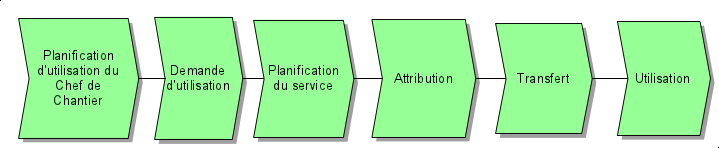
\includegraphics[width=15cm]{\PIXPATH/dcpv_utilisation_mat}
\end{center}
\subsubsection{Maintenance préventive}
\begin{center}
    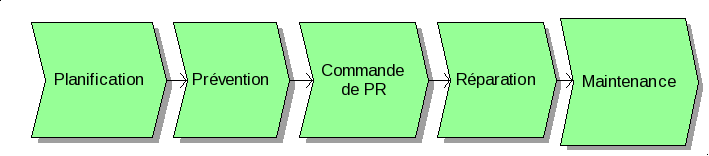
\includegraphics[width=15cm]{\PIXPATH/dcpv_maintenance_prev}
\end{center}
\subsubsection{Maintenance curative}
\begin{center}
    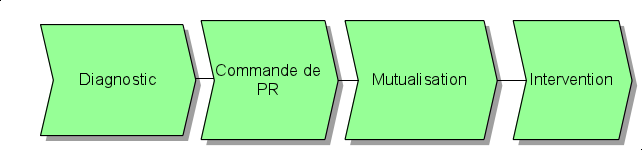
\includegraphics[width=15cm]{\PIXPATH/dcpv_maintenance_cur}
\end{center}

    % Fichier ./docs/tex/3-07-SP-MCT.tex

\section{Modèle conceptuel de traitements}

\subsection{Commande de pièces de rechange}

Le MCT est disponible dans le fichier {\sl Gstp-mct.pdf}.

Le responsable de chaque atelier émet une demande de pièce de rechange au
magasin le plus proche, qui ne sera délivrée qu'une fois par semaine.  La
livraison est faite par «zone chantier», c'est-à-dire qu'un camion est
responsable de desservir plusieurs ateliers qui sont proches les uns des autres
(30 km, par exemple). Cela réduit les coûts de livraison.
Si une demande est urgente, elle peut être délivrée plus rapidement
sans attendre les commandes des ateliers voisins.

Ateliers:
\begin{enumerate}
    \item Commande de pièce de rechange réalisée par un responsable atelier
\end{enumerate}

Magasin:
\begin{enumerate}
    \item Si le magasin ne possède pas les pièces nécessaires
    \begin{enumerate}
        \item Commande des pièces à un fournisseur
    \end{enumerate}

    \item Si la commande est urgente
    \begin{enumerate}
        \item Impression d'un avis de livraison
        (document utilisé pour confirmer la livraison)
        \item Livraison directe par camion
        Sinon
        \item Attente des commandes de tous les ateliers de la même zone
        \item Impression des avis de livraison
        \item Livraison par zone une fois par semaine
    \end{enumerate}
\end{enumerate}

À chaque fin de travaux dans un chantier ou à chaque nouveau chantier les
«zones chantiers» sont mises à jour. Un calcul est fait à partir des
distances entre les ateliers pour créer des zones où les chantiers sont
distants entre eux en moyenne de 30 km.


\subsection{Gestion des demandes de matériel}

%Dis que l'on garde le même processus, mais que l'on va numériser
%Précise les transferts entre chantiers

Le processus actuel est satisfaisant, et va donc être conservé. Il sera
toutefois numérisé, et formalisera les transferts de matériels entre
chantiers proches, à la fin d'un chantier et si le matériel ne nécessite
pas de maintenance lourde (effectuée au siège).


\subsection{Maintenance}

Le processus actuel est satisfaisant.

\subsection{Planification}

Le diagramme ne précise pas les différents intervenants ; on rappelle que :
\begin{itemize}
\item Chaque chef de chantier réalise avant le début du chantier un premier
planning d'utilisation de matériel;
\item Ce planning est transmis à la direction du matériel qui peut tenir à
jour un planning global et si nécessaire lancer des investissements (achat
de gros matériel).
\end{itemize}

\vskip 6pt

De plus, le MCT ne fait pas apparaître un point qui nous semble essentiel :
la correction du planning une fois le chantier lancé. Le chef de chantier
devrait réévaluer son planning d'utilisation de matériel au cours du
chantier, à raison d'une fois par mois. De cette manière, on sera à même de
mieux gérer l'utilisation du matériel et sa maintenance (si un matériel est
libéré plus tôt que prévu par exemple).


\subsection{Facturer les chantiers}

Il processus actuel est satisfaisant, cependant il manque un point essentiel,
la réactivité.

Il faudrait pouvoir gérer ou accéder aux informations de facturations en 
temps réel, plutôt que d’attendre l'édition de la facture au début du 
mois suivant.



    % Fichier ./docs/tex/3-08-SP-MCC.tex

%\section{Spécification du Système Cible}
\section{Modèle conceptuel de communication}

Le modèle de communication n'est pas changé. En effet nous ne bouleversons pas
les transactions entre les différents interlocuteurs. Nous modifierons les 
communications entre ces intervenants en les numérisant pour la plupart.
Cependant ces modifications n'interviennent pas dans le modèle conceptuel
de communication.

    % Fichier ./docs/tex/3-09-SP-MCD.tex

\section{Modèle conceptuel de données}

\subsection{Introduction}
Le MCD est disponible dans le fichier {\sl Gstp-mcd.pdf}.
Peu de modifications du MCD, simple ajout d'une classe {\emph commande standard}.

%Si le RQ est motivé il peut en faire un tableau....

\subsection{Ajout d'une classe Commande Standard}

La classe commande standard (STD\_CMD) représente des listes de pièces de 
rechange standard à commander à chaque début de chantier en fonction de son type.

\par{Description de l'entité}
\begin{description}
    \item[CODE-LISTE] Identifiant de la liste, TYPE : INT, LG : 10
    \item[NOM-LISTE] Nom de la liste de pièces, TYPE : STRING
    \item[DESC-LISTE] Description de la liste, TYPE : STRING
\end{description}

\par{Relations et cardinalité}
\begin{description}
    \item[COMM/LISTE]\el
         COMMANDE : Commande d'une liste standard (1,N)\el
        STD\_CMD : liste standard (0,N)
    \item[LISTE/PR]\el
         STD\_CMD : Liste des pièces de rechange (0,N)\el
        PIECE-RECHANGE :  Pièce de rechange.(0,N)
\end{description}

\subsection{Ajout d'une classe Planification Chantier}

La classe planification chantier (PLAN\_CHANTIER) représente les demandes
d'utilisation.

\par{Description de l'entité}
\begin{description}
    \item[CODE-DEMANDE] Identifiant de la commande, TYPE :INT, LG : 10
    \item[DESC-DEMANDE] Description de la demande, TYPE : STRING 
    \item[DATE-DEB]     Date début demande
    \item[DATE-FIN]     Date fin demande
\end{description}

\par{Relations et cardinalité}
\begin{description}
    \item[PLAN/CHANTIER]\el
        PLAN\_CHANTIER: planification d'un matériel pour un chantier (1,1)\el
        CHANTIER: chantier (0,N)
    \item[PLAN/MAT]\el
        PLAN\_CHANTIER: planification d'un matériel pour un chantier (0,1)\el
        CHANTIER: chantier (0,N)
\end{description}


% The end
\end{document}

